% Group addresses by affiliation; use superscriptaddress for long
% author lists, or if there are many overlapping affiliations.
% For Phys. Rev. appearance, change preprint to twocolumn.
% Choose pra, prb, prc, prd, pre, prl, prstab, prstper, or rmp for journal
%  Add 'draft' option to mark overfull boxes with black boxes
%  Add 'showpacs' option to make PACS codes appear
%  Add 'showkeys' option to make keywords appear
\documentclass[aps,
prd,
amsmath,
amssymb,
twocolumn,
%preprint,
floatfix,
groupedaddress]{revtex4-1}
%\documentclass[aps,prl,preprint,superscriptaddress]{revtex4-1}
%\documentclass[aps,prl,reprint,groupedaddress]{revtex4-1}
\usepackage{graphicx}% Include figure files
%\usepackage{float}
%\usepackage{stfloats}
%\usepackage{fixltx2e}
\usepackage{placeins}
\usepackage{dcolumn}% Align table columns on decimal point
\usepackage{amsmath}
\usepackage{amsthm, amsfonts, amssymb}
%\usepackage{supertabular}
\usepackage{array}
\usepackage{times}
\usepackage{latexsym}
\usepackage{hyperref}
\hypersetup{backref,  
%pdfpagemode=FullScreen,  
colorlinks=true,
linkcolor=red,
filecolor=red,
citecolor=blue}
\usepackage{epsfig}
\usepackage{subfigure}
% \usepackage{multicol}
%\usepackage{acronym}
%\usepackage[caption=false]{caption}
\usepackage{bm}% bold math
\usepackage{color}

\newcommand{\Sum}{\displaystyle\sum\limits}
\newcommand{\Int}{\displaystyle\int\limits}
\newcommand{\ii}{{\rm i}}
\newcommand{\D}{\mathrm{d}}
\newcommand{\eff}{\mathrm{eff}}
\newcommand{\phys}{\mathrm{phys}}
\newcommand{\real}{\mathrm{real}}
\newcommand{\peak}{\mathrm{peak}}
\newcommand{\EOB}{\mathrm{EOB}}
\newcommand{\NR}{\mathrm{NR}}
\newcommand{\RD}{\mathrm{RD}}
\newcommand{\Olap}{\mathcal{O}}
\newcommand{\MM}{\mathrm{MM}}
\newcommand{\EFF}{\mathrm{EFF}}
\newcommand{\X}{\mathrm{X}}
\newcommand{\Y}{\mathrm{Y}}
\newcommand{\Z}{\mathrm{Z}}
\newcommand{\horizon}{\mathrm{Horizon}}
\newcommand{\opt}{\mathrm{opt}}
\newcommand{\iso}{\mathrm{iso}}
\newcommand{\refr}{\mathrm{ref}}
\newcommand{\start}{\mathrm{start}}

\def\l({\left(}
\def\r){\right)}
%\def\l[{\left[}
%\def\r]{\right]}

\def\beq{\begin{equation}}
\def\eeq{\end{equation}}
\def\bea{\begin{eqnarray}}
\def\eea{\end{eqnarray}}
\def\nn{\nonumber}
\def\del{\partial}
\def\ola{\overleftarrow}
\def\ora{\overrightarrow}

% You should use BibTeX and apsrev.bst for references
% Choosing a journal automatically selects the correct APS
% BibTeX style file (bst file), so only uncomment the line
% below if necessary.
%\bibliographystyle{apsrev4-1}

\begin{document}

% Use the \preprint command to place your local institutional report
% number in the upper righthand corner of the title page in preprint mode.
% Multiple \preprint commands are allowed.
% Use the 'preprintnumbers' class option to override journal defaults
% to display numbers if necessary
%\preprint{}

%Title of paper
\title{Data Analysis with Effective-One-Body Waveforms - I}

% repeat the \author .. \affiliation  etc. as needed
% \email, \thanks, \homepage, \altaffiliation all apply to the current
% author. Explanatory text should go in the []'s, actual e-mail
% address or url should go in the {}'s for \email and \homepage.
% Please use the appropriate macro foreach each type of information

% \affiliation command applies to all authors since the last
% \affiliation command. The \affiliation command should follow the
% other information
% \affiliation can be followed by \email, \homepage, \thanks as well.
\author{Duncan A. Brown}
\email[]{dabrown@physics.syr.edu}
%\homepage[]{Your web page}
%\thanks{}
%\altaffiliation{}
\affiliation{Department of Physics, Syracuse University}

\author{Prayush Kumar}
\email[]{prkumar@syr.edu}
%\homepage[]{Your web page}
%\thanks{}
%\altaffiliation{}
\affiliation{Department of Physics, Syracuse University}

\author{Alex H. Nitz}
\email[]{ahnitz@syr.edu}
%\homepage[]{Your web page}
%\thanks{}
%\altaffiliation{}
\affiliation{Department of Physics, Syracuse University}

%Collaboration name if desired (requires use of superscriptaddress
%option in \documentclass). \noaffiliation is required (may also be
%used with the \author command).
%\collaboration can be followed by \email, \homepage, \thanks as well.
%\collaboration{}
%\noaffiliation

\date{\today}

\begin{abstract}

% insert abstract here
\end{abstract}

% insert suggested PACS numbers in braces on next line
\pacs{}
% insert suggested keywords - APS authors don't need to do this
%\keywords{}

%\maketitle must follow title, authors, abstract, \pacs, and \keywords
\maketitle

\section{Introduction}\label{sec:level1:Introduction}
Advanced LIGO will be up and operational from 2016 [citation], and advanced VIRGO from 2017 [citation]. The increase in the sensitivity of the advanced detectors is by almost an order of magnitude in measuring the gravitational-wave strain. This increases the volume of the visible universe by a factor of $\sim10^3$ \citep{LSCCBCRates2010}.

The fact that we can model the gravitational wave signals from coalescing compact binaries helps us extract information that is otherwise buried under instrumental noise. The technique of match-filtering is used to filter the detector against template waveforms, for this purpose. Detection searches done over the initial LIGO data used discrete banks of Taylor F2 waveform templates, that were accurate to 2PN \citep{LSCSearch2004,LSCSearch2005,LSCSearch2008}. The more recent effective-one-body approach \citep{EOBOriginalBuonannoDamour} to the two body problem has been highly developed in the recent past \citep{EOBNR01,EOBNRdevel01,EOBNRdevel02,EOBNRdevel03,EOBNRdevel04,EOBdevel01,EOBdevel02} to accurately model the gravitational waveforms from black-hole binaries. This approximant has been tuned against waveforms extracted from numerical relativity (NR) simulations, to increase the accuracy of the model further \citep{EOBNRdevel01,EOBNRdevel02,EOBNRdevel03,EOBNRdevel04}. The most recent EOB model \citep{
BuonannoEOBv2Main} has been calibrated against NR waveforms for 5 different mass-ratios.

In this paper, we investigate the gain in the sensitivity of the match-filtering searches for gravitaional waves from stellar-mass black-hole binaries, if done using the recent EOB model \citep{BuonannoEOBv2Main} to model the waveforms, instead of the Taylor F2 approximant. This was done by estimating the effective observation volume accesible to a match-filtering search, when done with each of the different waveform approximants. The details are presented in Sec.\ref{sec:level1:SearchVolume}. It was found that for systems with total mass greater than $18M_{\odot}$, match-filtering searches searching for gravitational wave signals for such systems could only be done viably using the full inspiral-merger-ringdown (IMR) EOB waveforms. Using any of the PN waveforms for this region would lead to greater than $10\%$ loss in the effective observation volume as compared to using the EOB waveforms. For binaries with total mass less than $\sim15M_{\odot}$, using the Taylor F2 approximant in a search leads to losses 
in observation volume below $10\%$. The stellar-mass black-hole binaries are taken to have individual component masses in the range $(3-20)M_{\odot}$.\newline

The detection searches in Initial LIGO data were done using discrete banks of waveform templates, that the detector data was filtered through \citep{LSCSearch2004,LSCSearch2005,LSCSearch2008}. In Sec.\ref{sec:level1:Effectualness}, we determine the portion of the designated component-mass region where the computationally cheaper PN approximants can be viably used for Advanced LIGO detection searches, and where in the same component-mass region can the same searches be viably done only with the EOB waveforms. This would give us an idea of how to divide the component-mass space for the future searches in detector data, and help us determine which approximant is to be used while searching in each sub-part of the designated component-mass space. For instance, the Taylor F2 waveforms are computationally very inexpensive to do the match-filtering searches with, as they are in frequency domain and the match-filtering is also done in the frequency domain, thus saving the dominant computational cost of fourier 
transforming time-domain waveforms [citation]. So, it would be preferable to use those from a computational budgeting point-of-view. We find out that for gravitational wave signals from binaries with total mass below $14M_{\odot}$, it suffices to use the Taylor F2 approximant. It was also found Taylor T4 [citation] approximant can be used in searching for signals from binaries with total mass below $12M_{\odot}$.\newline

Finally, the Owen-Sathya bank placement metric \citep{SathyaMetric2PN}\citep{SathyaBankPlacementTauN}, is used to place points in the component-mass space to form the bank of templates that the detection searches are done with. This metric was designed using Taylor F2 waveforms accurate to 2PN. We investigate in Sec.\ref{sec:level1:templateplacement} if this metric covers the component-mass space as required, with EOB waveform. Monte-Carlo study of the component-mass region reveals that using the Owen-Sathya metric results in undercovering the designated mass-region by almost $10\%$. If the bank were used, as such, with EOB waveforms, then the detection searches will lose event detection rate by upto $16\%$.
\section{Waveform Approximants}\label{sec:level1:WaveformApproximants}
\subsection{PN Approximants}\label{sec:level2:PNApproximants}
In this section, we present the basic equations that describe the dynamics of PN waveforms. 
In the adiabatic approximation, we can visualize the course of an inspiral as a series of radially shrinking circular orbits. 
And the radial coordinate evolves as the binary loses energy to gravitational radiation propagating outwards from the system.
For a binary with individual component masses $m_1$ and $m_2$ and total mass $M=m_1+m_2$, the conserved 3PN energy in terms of
its characteristic velocity $v$ can be written as
\begin{equation}
\begin{split}\label{eq:E3PN}
E_3(v)=&-\dfrac{1}{2}\eta v^2 \left[1- \l(\dfrac{3}{4}+\dfrac{1}{12}\eta\r)v^2 - \l(\dfrac{27}{8}-\dfrac{19}{8}\eta\right.\right.\\
+&\left.\left.\dfrac{1}{24}\eta^2 \r)v^4 - \l(\dfrac{675}{64}-\l(\dfrac{34445}{576}-\dfrac{205}{96}\pi^2\r)\eta\right.\right.\\
+&\left.\left.\dfrac{155}{96}\eta^2 +\dfrac{35}{5184}\eta^3\r) v^6\right],
\end{split}
\end{equation}
where $\eta=m_1m_2/(m_1+m_2)^2$ and $v=(\pi Mf)^{1/3}$, where $f$ stands for the frequency of the emitted gravitational wave throughout.
The gravitational flux from such a system, accurate to 3.5PN \citep{FluxandE3-5PN} is
\begin{equation}
\begin{split}\label{eq:Ft3.5PN}
F_{3.5}(v)=&\dfrac{32}{5}\eta^2 v^{10}\left[1 - \l(\dfrac{1247}{336}+\dfrac{35}{12}\eta\r)v^2+4\pi v^3\right.\\
-&\left.\l(\dfrac{44711}{9072}-\dfrac{9271}{504}\eta -\dfrac{65}{18}\eta^2 \r)v^4\right.\\
-&\left.\l(\dfrac{8191}{672}+\dfrac{583}{24}\eta\r)\pi v^5+ \l(\dfrac{6643739519}{69854400}\right.\right.\\
+&\left.\left.\dfrac{16}{3}\pi^2 -\dfrac{1712}{105}\gamma +\l(\dfrac{41}{48}\pi^2 -\dfrac{134543}{7776}\r)\eta \right.\right.\\
-&\left.\left.\dfrac{94403}{3024}\eta^2 -\dfrac{775}{324}\eta^3 -\dfrac{856}{105}\textrm{log}(16v^2)\r)v^6\right.\\ 
-&\left.\l(\dfrac{16285}{504}-\dfrac{214745}{1728}\eta -\dfrac{193385}{3024}\eta^2 \r)\pi v^7\right],
\end{split}
\end{equation}
where $\gamma$ is Euler's constant. If the change in the orbital frequency is much smaller than the frequency itself,
i.e. $\dot{\omega}/\omega \ll 1$, then we can approximate the energy of the system to be the energy averaged over a period.
The energy balance equation with the Kepler's Law give a couple of coupled differential equations for the evolution of the orbital phase,
\begin{subequations}\label{eq:PNOrbitalEvolution01}
\begin{align}
\dfrac{\D\phi}{\D t} - \dfrac{v^3}{M} &= 0,\label{eq:PNOrbitalEvolution01_01}\\
\dfrac{\D v}{\D t} + \dfrac{F(v)}{ME^{\prime}} &= 0;\label{eq:PNOrbitalEvolution01_02}
\end{align}
\end{subequations}
where the prime$(\prime)$ denotes $\D()/\D v$. We can also rewrite these as a pair of integral equations,
\begin{subequations}\label{eq:PNOrbitalEvolution02}
\begin{align}
t(v) &= t_{\refr} + M\Int_v^{v_{\refr}}\D v\dfrac{E^{\prime})}{F(v)},\label{eq:PNOrbitalEvolution02_01}\\
\phi(v) &= \phi_{\refr} + \Int_v^{v_{\refr}}\D v v^3\dfrac{E^{\prime}}{F(v)};\label{eq:PNOrbitalEvolution02_02}
\end{align}
\end{subequations}
where $t_{\refr}$ and $\phi_{\refr}$ are integration constants and $v_{\refr}$ is an arbitrary reference velocity.
We can use these constants to set the appropriate initial conditions for the generation of the inspiral.
%\subsection{Taylor T1}\label{sec:level3:Waveform:T1}
%If we substitute the expressions for the Energy of and flux from a particular system, exactly as they are from Eq.\eqref{eq:E3PN},\eqref{eq:Ft3.5PN} into Eq.\eqref{eq:PNOrbitalEvolution01}, and numerically solve it, the phase evolution thus obtained gives us the T1 waveform.
%
%Truncating the expression for Energy and flux at $n$PN order\citep{FluxandE3-5PN,PNFluxEnergy2PN,PNFluxEnergy3PN01,PNFluxEnergy3PN02}, results in a $n$PN template model\citep{CompTemplates2001,GW2PN}.
%
%The initial conditions for the inspiral are specified in terms of a particular starting gravitational wave frequency ($f_{start}$). This is incorporated by putting:
%\begin{align*}
%t_{ref} &= 0\\
%v_{ref} &= (\pi M f_{start})^{1/3}\\
%\phi_{ref} &= 0 \texttt{or} \pi/2
%\end{align*}
%
%giving us a pair of orthogonal templates, one corresponding to each value of $\phi_{ref}$.

%\subsubsection{Taylor T3}\label{sec:level2:TaylorT3}
%We start with explicitly inverting Eq.\eqref{eq:PNOrbitalEvolution02_01} to obtain $v(t)$, as a function of
%\begin{equation}
% \Theta = \l(\dfrac{v(t_{\refr}-t)}{5M}\r)^{-1/8}.
%\end{equation}
%From $v(t)$, we get $f(t)\equiv v(t)^3/(\pi M)$, which is the gravitational wave frequency at any instant of time during the course of the inspiral.
%The expression for $v(t)$ can be substituted in Eq.\eqref{eq:PNOrbitalEvolution02_02} to obtain $\phi(t)$. After this series of operations,
%we obtain the Taylor T3 gravitational phase and frequency as a function of time,
%\begin{subequations}
%\begin{align}
%\phi^{(T3)}_n(t) &= \phi^{(T3)}_{\refr} + \phi^t_n\Sum^{2n}_{k=0}C^{\phi}_k \Theta^k,\\
%f^{(T3)}_n(t) &= f^t_n\Sum^{2n}_{k=0}C^f_k \Theta^k,\label{eq:T3frequency}
%\end{align}
%\end{subequations}
%where $C^{\phi}_k$, $C^f_k$, $\phi^t_n$ and $f^t_N$ are constants,
%and the subscript $n$ stands for the post-Newtonian order to which the respective expression is accurate.
%Complete expressions for $\phi^{(T3)}_n(t)$ and $f^{(T3)}_n(t)$ can be obtained from Ref.\citep{CompTemplates2009}.
%To setup the initial conditions, one can solve Eq.\eqref{eq:T3frequency} for $t_{\refr}$, such that\newline
%$f^{(T3)}_n(0)=f_{\start}$.

\subsubsection{Taylor T4}\label{sec:level2:TaylorT4}
This approximant was originally proposed in Ref.\citep{TaylorT4Origin} and developed subsequently \citep{NRPNComparisonBaker2007,NRdynamicsq1,NRPNComparisonBoyleetal}.
We substitute the expression for energy from Eq.\eqref{eq:E3PN}, and the expression for flux from Eq.\eqref{eq:Ft3.5PN} into Eq.\eqref{eq:PNOrbitalEvolution01_02},
and expand $F(v)/ME^{\prime}(v)$ upto consistent PN order \citep{FluxandE3-5PN,PNFluxEnergy2PN,PNFluxEnergy3PN01,PNFluxEnergy3PN02,CompTemplates2001,GW2PN}.
The Eqns.\eqref{eq:PNOrbitalEvolution01} can subsequently be numerically solved to obtain the phase and gravitational-wave frequency as functions of time.
Thus we obtain the Taylor T4 phase evolution. The initial conditions for the inspiral are specified in terms of a particular starting gravitational-wave
frequency ($f_{\start}$). This is incorporated by putting
\begin{subequations}
\begin{align}
t_{\refr} &= 0,\\
v_{\refr} &= (\pi M f_{\start})^{1/3},\\
\phi_{\refr} &= 0\quad \textit{or}\quad \pi/2;
\end{align}
\end{subequations}
giving us a pair of orthogonal templates, one corresponding to either value of $\phi_{\refr}$.

\subsubsection{Taylor F2}\label{sec:level2:TaylorF2}
Using the stationary phase approximation, the gravitational waveform in the fourier domain can be approximated as
\begin{subequations}
\begin{align}
\tilde{h}(f) &= \dfrac{a(t(f))}{\sqrt{\dot{f}(t(f))}}e^{\ii \l(\Psi_f(t(f)) - \pi/4\r)},\\
\Psi_f(t) &\equiv 2\pi ft - 2\phi(t);
\end{align}
\end{subequations}
where $t(f)$ is the time at which the gravitational wave frequency $f$ becomes equal to the fourier frequency.
The expression for $t(f)$ (or $t(v)$) can be taken from Eq.\eqref{eq:PNOrbitalEvolution02_01}. And $\Psi_f$ can be obtained by solving Eqn.\eqref{eq:PNOrbitalEvolution01} written in frequency domain,
\begin{subequations}
\begin{align}\label{eq:PNF2Evolution01}
\dfrac{\D\Psi}{\D f}-2\pi t &= 0,\\
\dfrac{\D t}{\D f} + \dfrac{\pi M^2}{3v^2}\dfrac{E^{\prime}(v)}{F(v)} &=0.
\end{align}
\end{subequations}
This gives us the Taylor F2 waveform, that can be written as
\begin{equation}
\tilde{h}(f) = Af^{-7/6}e^{\iota\Psi(f)}.
\end{equation}
The amplitude $A\propto (m_1+m_2)^{5/6}\eta^{1/2}/\mathcal{R}$, where $\mathcal{R}$ is the distance to the binary. Upto 3.5PN order, the phase of the waveform 
\begin{equation}
\begin{split}\label{eq:PsiSPA}
\Psi(f)=&2\pi ft_c-\phi_c-\dfrac{\pi}{4} + \dfrac{3}{128}\dfrac{1}{\eta}v^{-5}\left[1 + \l(\dfrac{3715}{756} +\dfrac{55}{9}\eta\r)v^2\right.\\
-&\left. 16\pi v^3+\l(\dfrac{15293365}{508032}+\dfrac{27145}{504}\eta +\dfrac{3085}{72}\eta^2 \r)v^4\right.\\
+&\left.\l(\dfrac{38645}{756}-\dfrac{65}{9}\eta\r)\l(1+3\textrm{log}\l(\dfrac{v}{v_{\textrm{lso}}}\r)\r)\pi v^5\right.\\
+&\left.\left[\dfrac{11583231236531}{4694215680}-\dfrac{640}{3}\pi^2 -\dfrac{6848}{21}\gamma_E\right.\right.\\
-&\left.\left. \dfrac{6828}{21}\textrm{log}(4v)+\l(-\dfrac{15737765635}{3048192}+\dfrac{2255}{12}\pi^2 \r)\eta\right.\right.\\
+&\left.\left.\dfrac{76055}{1728}\eta^2 -\dfrac{127825}{1296}\eta^3\right] v^6\right.\\
+&\left.\l(\dfrac{77096675}{254016}+\dfrac{378515}{1512}\eta -\dfrac{74045}{756}\eta^2 \r)\pi v^7\right].
\end{split}
\end{equation}
The initial conditions are set by starting the waveform from a given starting gravitational-wave frequency, i.e. at $f=f_{\start}$.

\subsection{Effective-One-Body Approximant}\label{sec:level2:EOBNRv2}
With recent advancement in numerical relativity, there has been considerable development of the EOB waveform model \cite{EOBdevel01,EOBdevel02,EOBNRdevel03,DamourFluxhlm01,EOBNRdevel01}. We employ the EOB model proposed recently in Ref.\citep{BuonannoEOBv2Main}, which has been calibrated to NR waveforms for comparable mass binaries. This section summarizes the essential features of the model. Throughout, we will be using dimensionless units for all physical quantities, with $G=c=1$.

\subsubsection{The Hamiltonian}\label{sec:level3:EOBNRv2:Hamiltonian}
\textcolor{green}{Describe the effective and real hamiltonians. Describe the tuned parameters in the metric.}
The EOB approach maps the fully general-relativistic dynamics of the two-body system to that of an \textit{effective} mass moving in a deformed Schwarzschild spacetime \citep{EOBOriginalBuonannoDamour}. The physical dynamics is contained in the deformed-spacetime's metric coefficients, the EOB Hamiltonian \cite{EOBOriginalBuonannoDamour}, and the radiation-reaction force. Let $m_1$ and $m_2$ denote the masses of the two components of the binary system, with $m_1$ being the larger of the two. We define the total mass, the reduced mass, the mass-ratio and the symmetric mass-ratio as
\begin{equation}
M = m_1 + m_2, \,\mu =\dfrac{m_1m_2}{M},\, q=\dfrac{m_1}{m_2},\,\eta = \dfrac{\mu}{M};
\end{equation}
respectively. In polar coordinates $(r,\Phi)$, the EOB metric is written as
\begin{equation}
\D s_{\eff}^2 = -A(r)\D t^2 + \dfrac{A(r)}{D(r)}\D r^2 + r^2\left(\D\Theta^2 + \sin^2\Theta \D\Phi^2\right).
\end{equation}
The effective EOB Hamiltonian per unit reduced mass $\hat{H}^{\eff}$ can be written as \citep{EOBOriginalBuonannoDamour}
\begin{equation}
\hat{H}^{\eff} = \sqrt{A(r) \left( 1 +  \dfrac{A(r)}{D(r)}p_r^2 + 2(4 - 3\eta)\eta \dfrac{p_r^4}{r^2} + \dfrac{p^2_{\Phi}}{r^2} \right)},
\end{equation}
where $(p_r,p_{\Phi})$ are momenta conjugate to $(r,\Phi)$ respectively. This effective Hamiltonian describes the geodesic dynamics of the \textit{effective} mass \citep{EOBEffHamiltonian}. It is found convenient to replace the radial momentum $p_r$, with the momentum conjugate to the EOB extension of the Regge-Wheeler \textit{tortoise} radial coordinate $r_*$, where $r_*\equiv\int\sqrt{D(r)}/A(r)\,\D r$ \citep{DamourNQC01} . This momentum coordinate $p_{r_*}$ is related to $p_r$ as,
\begin{equation}
p_{r_*} = \dfrac{A(r)}{\sqrt{D(r)}}\,p_r.
\end{equation}
In $\l(r,\Phi,p_{r_*},p_{\Phi}\r)$ coordinates, the effective Hamiltonian can so be written as \citep{BuonannoEOBv2Main},
\begin{equation}
\hat{H}^{\eff} = \sqrt{p^2_{r_*} + A(r) \left( 1 + 2(4 - 3\eta)\eta \dfrac{p_{r_*}^4}{r^2} + \dfrac{p^2_{\Phi}}{r^2} \right)}.
\end{equation}
The EOB Hamiltonian (labelled the \textit{real} Hamiltonian), that describes the conservative dynamics of the binary,  is related to the effective Hamiltonian as (per unit reduced mass),
\begin{equation}
\hat{H}^{\real} = \dfrac{1}{\eta} \sqrt{1 + 2\eta (\hat{H}^{\eff} - 1)}.
\end{equation}
The metric coefficients $A(r)$ and $D(r)$ were originally calculated as taylor expansions \cite{EOBOriginalBuonannoDamour,PadeAD}. At PN order $n$:
\begin{eqnarray}
A(r) = \Sum^{n+1}_{i=0} \dfrac{a_i (\eta)}{r^i},\quad
D(r) = \Sum^{n}_{i=0} \dfrac{d_i (\eta)}{r^i};
\end{eqnarray}
where currently $A(r)$ and $D(r)$ are known to 3PN order $\l(n=3\r)$.  The EOB model that we use employs Pade-resummations of the taylor expansions of these coefficients \citep{BuonannoEOBv2Main}. The use of re-summation techniques to express their taylor expansions as ratios of polynomials was proposed to ensure the existence of the innermost stable circular orbit in the EOB framework \citep{PadeAD}. For $A(r)$, we use its Pad\'{e} re-summation at order $(1,5)$, while for $D(r)$, we use the re-summation  at order $(0,3)$ \citep{BuonannoEOBv2Main}, such that
\begin{eqnarray*}
D(r) &=& \dfrac{r^3}{(52\eta - 6\eta^2) + 6\eta r + r^3},\\
A(r) &=& \dfrac{\alpha_0 r^5 + \alpha_1 r^4}{\beta_0 r^5 + \beta_1 r^4 + \beta_2 r^3 + \beta_3 r^2 + \beta_4 r +\beta_5};
\end{eqnarray*}
where,
\begin{equation}
\begin{split}
\alpha_0 &= 32 - 4a_4 - a_5 - 24\eta ,\\
\alpha_1 &= -64 + 12a_4 + 4a_5 + a_6 + 64\eta - 4\eta^2 ,\\
\beta_0 &= 32 - 4a_4 - a_5 - 24\eta ,\\
\beta_1 &= 4a_4 + 2a_5 + a_6 + 16\eta - 4\eta^2 ,\\
\beta_2 &= 8a_4 + 4a_5 + 2a_6 + 32\eta - 8\eta^2 ,\\
\beta_3 &= 16a_4 + 8a_5 + 4a_6 + \left(8a_4 + 2a_5\right)\eta + 32\eta^2 ,\\
\beta_4 &= 4a_4^2 + a_4a_5 + 16a_5 + 8a_6\\ 
             &+ \left(32a_4 - 2a_6\right)\eta + 32\eta^2 + 8\eta^3 ,\\
\beta_5 &= 4a_4^2 + 4a_4a_5 + a+5^2 - a_4a_6 + 16a_6\\
             &+ \left(32a_4 + 16a_5 - 8a_6\right)\eta + 4a_4\eta^2 + 32\eta^3 ,\\
\end{split}
\end{equation}
and,
\begin{subequations}\label{metric_tunable_coeffs}
\begin{align}
a_4 &= \left(\dfrac{94}{3} - \dfrac{41}{32}\pi^2\right)\eta ,\\
a_5 &= \left(-5.828 - 143.5\eta + 447\eta^2\right)\eta ,\\
a_6 &= 184\eta .
\end{align}
\end{subequations}
To have the dynamics agree more closely with NR simulations, the coefficients $a_5$, $a_6$ were introduced and thence calibrated for comparable mass binaries \citep{EOBNRdevel01,EOBNRdevel02,EOBNRdevel03,EOBNRdevel04}. The values for $a_5$ and $a_6$ that we use here are those that were found in Ref.\citep{BuonannoEOBv2Main}, where they have calibrated the EOB dynamics to numerical simulations for five different value of mass-ratio $(q)$.

\subsubsection{Initial Conditions}\label{sec:level3:EOBNRv2:IniCond}
\textcolor{green}{Describe how one goes from (f0,m1,m2) to (q0,p0)}
To evolve the dynamics of the binary system, from the Hamiltonian, we need to specify the coordinate configuration that the system starts out in. For a generic precessing black-hole binary, an adiabatic expression of radiation-reaction is derived with the approximate picture that the binary inspirals over a sequence of spherical orbits, shrinking in the radial direction. In the absence of radiation-reaction, the conditions for motion on spherical orbits have been calculated in Ref.\cite{IniConditions-precessing}. We take their non-spinning limit to define the initial configuration of the binary, requiring
\begin{subequations}
\begin{align}\label{eq:IniHr}
\dfrac{\partial\hat{H}^{\real}}{\partial r} &= 0,\\ \label{eq:IniHpr}
\dfrac{\partial\hat{H}^{\real}}{\partial p_{r_*}} &= \dfrac{1}{\eta}\dfrac{\D E}{\D t}\dfrac{(\partial^2\hat{H}^{\real}/\partial r\partial p_{\Phi} )}{(\partial\hat{H}^{\real}/\partial p_{\Phi})(\partial^2\hat{H}^{\real}/\partial r^2)}, \\\label{eq:IniHpphi}
\dfrac{\partial\hat{H}^{\real}}{\partial p_{\Phi}} &= \hat{\Omega}_0,
\end{align}
\end{subequations}
where $\hat{\Omega}_0 = \pi Mf_0$, with $f_0$ being the starting gravitational wave frequency. Simplifying Eq.\eqref{eq:IniHr}, and ignoring the terms involving $p_{r_*}$, we get a relation between $p_{\Phi}$ and $r$:
\begin{equation}
p_{\Phi}^2 = \dfrac{r^3A'(r)}{2A(r) - rA'(r)} \\ \label{eq:Inipphi},
\end{equation}
where the prime($'$) denotes $\partial/\partial r$. Substituting this in Eq.\eqref{eq:IniHpphi}, we get the relation:
\begin{equation}
\dfrac{A'(r)}{2r(1 + 2\eta(\hat{H}^{\eff} - 1))} = \hat{\Omega}_0^2.\\ \label{eq:Inir}
\end{equation} 
Thus, between Eq.\eqref{eq:Inir} and Eq.\eqref{eq:Inipphi}, we get the initial values of $(r, p_{\Phi})$, corresponding to the initial gravitational wave frequency $f_0$. These values can be substituted into Eq.\eqref{eq:IniHpr}, to numerically solve for the initial value of $p_{r_*}$, thereby completely specifying the starting coordinate configuration of the binary system. 
%Eq(\ref{eq:IniHpr}) can be expanded to:
%
%\begin{equation}
%\dfrac{\l( \l(1+2\eta\l(\hat{H}_{eff} - 1\r)\r)\dfrac{\partial^2\hat{H}_{eff}}{\partial r^2} - \eta\l(\dfrac{\partial\hat{H}_{eff}}{\partial r}\r)^2 \r) \dfrac{\partial\hat{H}_{real}}{\partial p_{\Phi}}\dfrac{\partial\hat{H}_{real}}{\partial p_{r_*}}}{\l(1+2\eta\l(\hat{H}_{eff} - 1\r)\r) \l(\l(1+2\eta\l(\hat{H}_{eff} - 1\r)\r) \dfrac{\partial^2\hat{H}_{eff}}{\partial r \partial p_{\Phi}} - \eta\dfrac{\partial\hat{H}_{real}}{\partial p_{\Phi}}\dfrac{\partial\hat{H}_{real}}{\partial p_{r_*}} \r) } = \dfrac{1}{\eta}\dfrac{dE}{dt}
%\end{equation}

\subsubsection{Gravitational Flux}\label{sec:level3:Flux}
\textcolor{green}{Describe how the flux is written as a summation over the waveform multipoles, and how each multipole is defined and factorized. Describe each factor. Say that N22=something, and other Nlm =1, describing them in detail later.}
The propagating gravitational waves carry out energy with them, causing a radiation-reaction force on the binary. This force causes the orbits to evolve radially, and is related to the flux of energy ($E$) as
\begin{equation}
\hat{F}_{\Phi} = -\dfrac{1}{\eta \hat{\Omega}} \dfrac{\D E}{\D t} = -\dfrac{1}{\eta v_{\Omega}^3} \dfrac{\D E}{\D t},
\end{equation}
where, $v_{\Omega}=(\hat{\Omega})^{1/3}=(\pi Mf)^{1/3}$ and $f$ is the instantaneous gravitational wave frequency. The flux of energy, $\D E/\D t$, is obtained by summing up the contribution to it from each of the propagating waveform multipole.
\begin{equation}
\frac{\D E}{\D t} = \frac{\hat{\Omega}^2}{8\pi} \Sum_{l}\Sum_{m} \left|\frac{\mathcal{R}}{M} h_{lm}\right|^2,
\end{equation}
where $\mathcal{R}$ is the physical distance to the binary (throughout), and $h_{lm}$ are the multipoles of the waveform, implicitly defined by the decomposition
\begin{equation}
h_+ + \ii h_{\times} = \dfrac{M}{\mathcal{R}} \Sum^{\infty}_{l=2} \Sum^{m=l}_{m = -l} S^{lm}_{-2} h_{lm},
\end{equation}
where $S^{lm}_{-2}$ is the $(l,m)$-th spin $(-2)$ weighted spherical harmonic, and $h_+$ and $h_{\times}$ denote the two orthogonal polarizations of gravitational waves from a binary. The taylor expansions of these $h_{lm}$ multipoles have been re-summed as products of individually re-summed factors \citep{DamourFluxhlm01}. It has been shown \citep{EOBNRdevel01,EOBNRdevel02} that this factorized-re-summation of the multipoles enhances the agreement with waveform multipoles extracted from NR simulations \citep{EOBNR01}. We can write each factorized-re-summed multipole as \citep{DamourFluxhlm01}
\begin{subequations}\label{eq:hNoNQC}
\begin{align}
h_{lm} &= h^F_{lm} N_{lm}\\
h^F_{lm} &= h^{(N,\epsilon)}_{lm} \hat{S}_{\eff}^{(\epsilon)} T_{lm} \exp^{\ii\delta_{lm}} (\rho_{lm})^l,
\end{align}
\end{subequations}
where $\epsilon$ is $0$ if $\l(l+m\r)$ is even, and is $1$ otherwise. The first factor $h^{(N,\epsilon)}_{lm}$ is the re-summation of the Newtonian order contribution in $h^F_{lm}$, and can be written as \citep{DamourFluxhlm01},
\begin{equation}\label{eq:hNewtonian}
h^{(N,\epsilon)}_{lm} = \dfrac{M}{\mathcal{R}}\eta\,n_{lm}^{(\epsilon)}\,c_{l+\epsilon}(\eta)\,V^l_{\Phi}\,Y^{l-\epsilon,-m}\left(\dfrac{\pi}{2},\Phi\right).
\end{equation}
The first two sub-factors in the Newtonian term \citep{BuonannoEOBTerms};
\begin{subequations}
\begin{align}
n^{(\epsilon=0)}_{lm} &= (\ii m)^l \dfrac{8\pi}{(2l+1)!!}\sqrt{\dfrac{(l+1)(l+2)}{l(l-1)}} ,\\
n^{(\epsilon=1)}_{lm} &= -(\ii m)^l \dfrac{16\pi \ii}{(2l+1)!!}\sqrt{\dfrac{(2l+1)(l+2)(l^2-m^2)}{(2l-1)(l+1)l(l-1)}},
\end{align}
\end{subequations}
and
\begin{equation}
\begin{split}
c_{l+\epsilon} &= \left( \dfrac{1}{2} - \dfrac{1}{2}\sqrt{1-4\eta} \right)^{l+\epsilon-1} \\
						&+ (-1)^{l+\epsilon}\left( \dfrac{1}{2} + \dfrac{1}{2}\sqrt{1-4\eta} \right)^{l+\epsilon-1},
\end{split}
\end{equation}
are constant scaling factors that depend only on $l$ and $m$. The sub-factor $V_{\Phi}$ captures the dependence of the Newtonian order amplitude on the characteristic velocity of the binary $v_{\Omega}$, such that 
\begin{subequations}
\begin{align}
V_{\Phi}^l &= v_{\Phi}^{(l+\epsilon)},\quad &(l,m) \neq (2,1) , (4,4),\\
V_{\Phi}^l &= \dfrac{1}{r_{\Omega}}v_{\Phi}^{(l+\epsilon-2)},\quad &(l,m) = (2,1) , (4,4);
\end{align}
\end{subequations}
where,
\begin{eqnarray}
v_{\Phi} \equiv & v_{\Omega}^3 r_{\Omega},\\
r_{\Omega} \equiv & r\left[ \dfrac{2\left(1+2\eta\left(\sqrt{A(r)(1+p_{\Phi}^2/r^2)} -1 \right) \right)}{r^2dA(r)/dr} \right]^{1/3}.
\end{eqnarray}
The $v_{\Omega}$ dependence of the amplitude, encoded in $V_{\Phi}$, is expressed differently for $h_{21}$ and $h_{44}$ than for other multipoles for reasons given in Sec. III E of Ref.\citep{BuonannoEOBv2Main}. The last sub-factor in the Newtonian term, $Y^{l,m}$, is the $(l,m)$-th scalar spherical harmonic.

Further, $\hat{S}_{\eff}^{(\epsilon)}$ is the $\mu$-normalized source term, whose definition comes from the EOB formalism \citep{DamourFluxhlm01,BuonannoEOBTerms}. In the case of even-$\l(l+m\r)$, the source term is given by the mass moments, and for the odd-$\l(l+m\r)$ case, its given by the current moments \citep{BuonannoEOBTerms} of the binary,
\begin{subequations}
\begin{align}
\hat{S}_{\eff}^{(\epsilon=0)} &= \hat{H}^{\eff}(r,p_{r_*},p_{\Phi}) ,\\
\hat{S}_{\eff}^{(\epsilon=1)} &= \hat{L}_{\eff} = p_{\Phi} v_{\Omega}.
\end{align}
\end{subequations}
The "tail term" $T_{lm}$ is the re-summation of the leading order logarithmic terms that enter into the transfer function of the near-zone multipolar waves to the far-zone \citep{BuonannoEOBTerms},
\begin{equation}
\begin{split}
T_{lm} =& \dfrac{\Gamma(l+1-2\ii m\,\eta\,\hat{H}^{\real}\hat{\Omega})}{\Gamma(l+1)} \exp\left[\pi\,m\,\eta\,\hat{H}^{real}\hat{\Omega}\right]\\
             &\times  \exp\left[ 2\ii\,m\,\eta\,\hat{H}^{\real} \hat{\Omega}\mathrm{log}_e(4\,m\,\hat{\Omega}/\sqrt{e}) \right];
\end{split}
\end{equation}
where $\Gamma()$ is the gamma function. The sub-leading dephasing effects between the near-zone multipolar waves and the far-zone waves are re-summed into $\delta_{lm}$ \citep{BuonannoEOBTerms}. The values for $\delta_{lm}$ can be read off from Eqns.[B1a - B6d] of Ref.\citep{BuonannoEOBv2Main}. The last term $\rho_{lm}$ is the complex ratio of the PN expansions of $h_{lm}$ to the product of all factors (other than $\rho_{m}$ itself) that constitute $h^F_{lm}$, given in Eq.\eqref{eq:hNoNQC}. For different values of $l$ and $m$, the expressions for $\rho_{lm}$ are given in Eqns.[B9a - B14g] of Ref.\citep{BuonannoEOBv2Main}. This model also has a few free parameters in the expressions for $\delta_{lm}$ and $\rho_{lm}$, i.e. $\rho^{(6)}_{21}$,$\rho^{(6)}_{33}$,$\rho^{(6)}_{44}$,$\rho^{(6)}_{55}$,$\delta^{(7)}_{21}$,$\delta^{(7)}_{33}$,$\delta^{(5)}_{44}$ and $\delta^{(5)}_{55}$ as they appear in Eqns.[B9b,B10a,B11a,B12a,B1b,B2a,B3a,B4a] of Ref.\citep{BuonannoEOBv2Main}. These parameters are all set to zero in 
the calculation of energy flux while generating the EOB dynamics.

And lastly, $N_{lm}$ is the factor that attempts to capture the non-circularity of the orbits,
\begin{equation}\begin{split}\label{eq:Nlmdef}
N_{lm} =& \left[1 + \dfrac{p_{r_*}^2}{(r\hat{\Omega})^2} \left( a_1^{h_{lm}} + \dfrac{a_2^{h_{lm}}}{r} + \dfrac{a_3^{h_{lm}}}{r^{3/2}} \right)\right] \\
&\times \exp\left[\ii \left( b_1^{h_{lm}} \dfrac{p_{r_*}}{r\hat{\Omega}} + b_2^{h_{lm}} \dfrac{p_{r_*}^3}{r\hat{\Omega}} \right) \right].
\end{split}\end{equation}
where $(r,p_{r_*})$ are the radial coordinate and momentum conjugate to the \textit{tortoise} radial coordinate, respectively, and $\hat{\Omega}$ is the dimensionless instantaneous gravitational wave frequency. To calculate the energy flux, following the prescription of Ref.\citep{BuonannoEOBv2Main}, we set
\begin{subequations}
\begin{align}
a_1^{h_{22}} &= -4.559 + 18.76\eta - 24.23\eta^2, \\
a_2^{h_{22}} &= 37.68 - 201.5\eta + 324.6\eta^2, \\
a_3^{h_{22}} &= -39.6 + 228.9\eta - 387.2\eta^2,
\end{align}
\end{subequations}
$a_i^{h_{lm}}=0$ for $(l,m)\neq(2,2)$, and $b_i^{h_{lm}}=0$. This amounts to including the non-quasi-circular corrections only for the leading order $(l,m)=(2,2)$ multipole alone in the flux.
 
\subsubsection{Evolution of Dynamics}\label{sec:level3:DynamicalEvolution}
\textcolor{green}{Describe how, starting from the initial conditions, the entire dynamics is evolved, and how we get hFlm(t)}
By now, we have all the ingredients necessary to evolve the EOB dynamics and generate the waveform. With the EOB Hamiltonian and the gravitational flux constructed, we can write the equations of motion,
\begin{eqnarray}
\dfrac{\D r}{\D\hat{t}} &=& \dfrac{A(r)}{\sqrt{D(r)}}\dfrac{\partial \hat{H}^{\real}}{\partial p_{r*}} (r, p_{r*}, p_{\Phi}) ,\\
\dfrac{\D\Phi}{\D\hat{t}} &\equiv & \hat{\Omega} = \dfrac{\partial \hat{H}^{\real}}{\partial p_{\Phi}} (r, p_{r*}, p_{\Phi}) , \\ 
\dfrac{\D p_{r_*}}{\D\hat{t}} &=& -\dfrac{A(r)}{\sqrt{D(r)}} \dfrac{\partial \hat{H}^{\real}}{\partial r} (r, p_{r*}, p_{\Phi}) ,\\
\dfrac{\D p_{\Phi}}{\D\hat{t}} &=& \hat{F}_{\Phi}(r, p_{r*}, p_{\Phi}) ;
\end{eqnarray}
where, $\hat{t}\,(\equiv t/M)$ is time in dimensionless units. Starting from the initial coordinate configuration calculated for a fiducial starting gravitational wave frequency, we numerically integrate these equations to get the evolution of various coordinates and momenta over the course of inspiral, i.e.$(r(t),\Phi(t),p_r(t),p_{\Phi}(t))$, till the EOB light-ring. We also get $h^F_{lm}(t)$ by the integration of these equations. While generating the $h^F_{lm}(t)$ from the dynamics, the free parameters in the expressions for $\delta_{lm}$ and $\rho_{lm}$, i.e. $\rho^{(6)}_{21}$,$\rho^{(6)}_{33}$,$\rho^{(6)}_{44}$,$\rho^{(6)}_{55}$,$\delta^{(7)}_{21}$,$\delta^{(7)}_{33}$,$\delta^{(5)}_{44}$ and $\delta^{(5)}_{55}$ as they appear in Eqns.[B9b,B10a,B11a,B12a,B1b,B2a,B3a,B4a] of Ref.\citep{BuonannoEOBv2Main}, are set to their prescribed values given in Eqn.[38a-19b] of Ref.\citep{BuonannoEOBv2Main}. These parameters were calibrated against NR simulations, to maximize the phase and amplitude agreement between 
the EOB waveform multipoles and the NR waveform multipoles.

\subsubsection{Constructing the waveform multipoles}\label{sec:level3:hlm}
\textcolor{green}{Describe how the hFlm is used to get Nlm, and then hlm(t) is calculated.}
The novel feature of this EOB model is that it has the factor $N_{lm}$ in the expression of the waveform multipoles (as in Eq.\eqref{eq:hNoNQC}), that attempts to capture the non-circularity of the orbits as the objects enter the late-inspiral stage where the approximation of treating the orbits as quasi-circular, becomes inaccurate. As mentioned before, with this non-quasi-circular factor $N_{lm}$, we write the waveform multipoles as
\begin{equation}
h_{lm} = h^F_{lm} N_{lm}
\end{equation}
where, $h^F_{lm}$ is the factorized-re-summed version of the gravitational wave modes defined above in Eq.\eqref{eq:hNoNQC}. It is perhaps worth mentioning, that, in previous works \citep{EOBdevel02,EOBNRdevel04}, a factor to similar purpose was introduced into the expression for the energy flux. Introducing $N_{lm}$ in the expression of the waveform multipoles \citep{DamourNQC01,BuonannoEOBv2Main}, has a dual advantage as these multipoles figure both in the equations of motion of the system, and the waveform itself.
%\begin{equation}\begin{split}\label{eq:Nlmdef}
%N_{lm} =& \left[1 + \dfrac{p_{r_*}^2}{(r\hat{\Omega})^2} \left( a_1^{h_{lm}} + \dfrac{a_2^{h_{lm}}}{r} + \dfrac{a_3^{h_{lm}}}{r^{3/2}} \right)\right] \\
%&\times \exp\left[\ii \left( b_1^{h_{lm}} \dfrac{p_{r_*}}{r\hat{\Omega}} + b_2^{h_{lm}} \dfrac{p_{r_*}^3}{r\hat{\Omega}} \right) \right],
%\end{split}\end{equation}
In $N_{lm}$, there are free parameters $a_i^{h_{lm}}$ and $b_i^{h_{lm}}$, that need to be uniquely determined for each binary system, using input from numerical relativity simulations. For each set of $(l,m)$ we have 5 of these unknown parameters, and so we need 5 conditions to determine them uniquely. It was observed \citep{BuonannoEOBv2Main} that the time at which the orbital frequency ($\Omega$) peaks, coincides with the time at which the amplitude of the dominant mode $|h_{22}|$ peaks. Other waveform multipoles have their amplitudes peak slightly before or after that time. Lets define
\begin{equation}
\Delta t^{lm}_{\peak} = t^{lm}_{\peak} - t^{\Omega}_{\peak}.
\end{equation}
Since $\Omega$ peaks at the same time as $h_{22}$ peaks in amplitude,
\begin{equation}
t^{\Omega}_{\peak} = t^{22}_{\peak}
\end{equation}
The values for $\Delta t^{lm}_{peak}$ can be read off from Table III in Ref.\citep{BuonannoEOBv2Main}. Requiring that the amplitude of each of the multipole peak at the time predicted by NR (i.e. at time $t^{\Omega}_{\peak}+\Delta t^{lm}_{\peak}$), and that its first and second time-derivatives match the values given by NR (at the time at which the amplitude peaks), gives us the three $a_i^{h_{lm}}$ parameters.  (the conditions given in Eqns.\eqref{eq:NQCa1}-\eqref{eq:NQCa3}). Requiring that the frequency and the first time-derivative of the frequency of each multipole match the value of the frequency given by NR, at the time at which the amplitude of the respective multipole peaks, gives us the remaining two $b_i^{h_{lm}}$ phase parameters (Eqns.\eqref{eq:NQCb1}-\eqref{eq:NQCb2}).
\begin{subequations}
\begin{align}
\left| h^{\EOB}_{lm}(t^{\Omega}_{\peak}+\Delta t^{lm}_{\peak}) \right| &=& \left|h^{\NR}_{lm}(t^{lm}_{\peak})\right|\label{eq:NQCa1},\\
\dfrac{\D\left| h^{\EOB}_{lm} \right|}{\D t}(t^{\Omega}_{\peak}+\Delta t^{lm}_{\peak})  &=& \dfrac{\D\left|h^{\NR}_{lm}\right|}{\D t}(t^{lm}_{\peak})\label{eq:NQCa2},\\
\dfrac{\D^2\left| h^{\EOB}_{lm}\right|}{\D t^2}(t^{\Omega}_{\peak}+\Delta t^{lm}_{\peak})  &=& \dfrac{d^2\left|h^{\NR}_{lm}\right|}{\D t^2}(t^{lm}_{\peak})\label{eq:NQCa3},\\
\omega^{\EOB}_{lm}(t^{\Omega}_{\peak}+\Delta t^{lm}_{\peak}) &=& \omega^{\NR}_{lm}(t^{lm}_{\peak})\label{eq:NQCb1},\\
\dfrac{\D\omega^{\EOB}_{lm}}{\D t}(t^{\Omega}_{\peak}+\Delta t^{lm}_{\peak})  &=& \dfrac{\D\omega^{\NR}_{lm}}{\D t}(t^{lm}_{\peak})\label{eq:NQCb2}.
\end{align}
\end{subequations}
These conditions ensure that the behaviour of each of the waveform multipole matches the behaviour predicted by NR simulations accurately, at the time of peak of the gravitational wave frequency. As the quasi-normal-modes (QNMs) of the ringdown part of the waveform are attached to the inspiral-plunge waveform at this point in time, the conditions on the time-derivative of the amplitude and frequency (Eqns.\eqref{eq:NQCa2}-\eqref{eq:NQCa3},\eqref{eq:NQCb2}) also ensure consistency in the attachment of the ringdown QNMs.

\subsubsection{Ringdown}\label{sec:level3:RD}
\textcolor{green}{Describe the ringdown attachment procedure.}
The EOB merger-ringdown waveform is modelled as \citep{EOBNRdevel01,EOBNRdevel02,EOBNRdevel04,EOBNRdevel04}
\begin{equation}
h_{lm}^{\RD}(t) = \Sum^{N-1}_{n=0}A_{lmn}e^{-\ii\sigma_{lmn}(t-t_{lm}^{\mathrm{match}})},
\end{equation}
where $N$ is the number of the QNMs that one models the merger-ringdown signal as the linear combination of (for our model, $N=8$); $t_{lm}^{\mathrm{match}}$ is chosen to be the time at which the amplitude of the inspiral part of $h_{lm}(t)$ peaks ($t^{lm}_{\peak}$)\citep{EOBNRdevel01,BuonannoEOBv2Main} and $\sigma_{lmn}$ are complex frequencies of these modes that depend on the final black-hole mass and spin \citep{BHRDQNMs}. The final black-hole that is formed after the coalescence of the two objects, has a mass $M_f$ and spin $a_f$, that can be determined from the physical parameters of the binary as \citep{BuonannoEOBv2Main},
\begin{subequations}
\begin{align}
\dfrac{M_f}{M} &= 1 + \l(\sqrt{\frac{8}{9}}-1\r)\eta - 0.4333\eta^2 - 0.4392\eta^3,\\
\dfrac{a_f}{M} &= \sqrt{12}\eta - 3.871\eta^2 + 4.028\eta^3,
\end{align}
\end{subequations}
and these relations are the same as Eqn.(28a-28b) of Ref.\citep{BuonannoEOBv2Main}.

$A_{lmn}$ are complex amplitudes, that are determined by a hybrid-comb numerical matching procedure described in detail in Sec.II C of Ref.\citep{BuonannoEOBv2Main}. Ending at $t=t_{lm}^{\mathrm{match}}$, a small time interval $\Delta t^{\mathrm{match}}_{lm}$ is taken. For values of $\Delta t^{\mathrm{match}}_{lm}$, see Table III of Ref.\citep{BuonannoEOBv2Main}. This time interval is divided evenly into $N-3$ subdivisions. The amplitudes of the inspiral waveform and the merger-ringdown waveform are equated at the $N-2$ points, bounding these $N-3$ subdivisions of the time interval $\left[t_{lm}^{\mathrm{match}}-\Delta t^{\mathrm{match}}_{lm},t_{lm}^{\mathrm{match}}\right]$. At the first and the last point in this time interval, the time-derivatives of the amplitude of the inspiral waveform and the merger-ringdown waveform are also equated, giving us $2$ more constraints on $A_{lmn}$. With a total of $(N-2)+2=N$ constraints, all the $N$ complex $A_{lmn}$ can be uniquely determined.

\subsubsection{Final Waveform}\label{sec:level3:FinalWaveform}
\textcolor{green}{Describe how h+ and hx are obtained from hlm and ringdown}
In the previous few subsections we describe the generation of the the inspiral-merger-ringdown EOB waveform multipoles $h_{lm}$. These can be combined to give the two orthogonal polarizations of the gravitational waveform, $h_+$ and $h_{\times}$, 
\begin{equation}
h_+ + \ii h_{\times} = \dfrac{M}{\mathcal{R}} \Sum^{\infty}_{l=2} \Sum^{m=l}_{m = -l} S^{lm}_{-2}(\iota,\theta) h_{lm},
\end{equation}
where $S^{lm}_{-2}$ is the $(l,m)$-th spin $(-2)$ weighted spherical harmonic, $\iota$ is the inclination angle  that the binary's angular momentum makes with the line of sight, and $\theta$ is a fiducial phase angle.

%\subsubsection{Inspiral and plunge: Dynamics}\label{sec:level3:InspiralEOBDynamics}
%These parts of the model have been tuned separately to model NR waveforms accurately \citep{EOBNRdevel01,DamourFluxhlm01,BuonannoEOBv2Main}.

 
%\subsubsection{Inspiral and plunge: Multipolar Waveform}\label{sec:level3:Waveform:EOB:MultipolarWaveform}

%\subsubsection{Merger-Ringdown}\label{sec:level2:WaveformEOBRD}

%\subsubsection{Initial Conditions}\label{sec:level2:Waveform:EOB:InitialConditions}


\section{EOB: Gain in Search Volume}\label{sec:level1:SearchVolume}
We compare the sensitivity of match-filtering searches, in terms of the effective observation volume available to them, using the different waveform approximants described in the Sec.\ref{sec:level1:PNApproximants}. One can think of the effective observation volume as the (effective) spacial volume centered at the gravitational wave detector, within which, all binary systems emitting gravitational radiation will be detected with a signal-to-noise ratio (SNR) higher than $8$, by the match-filter. In the advanced detector era, it is expected that we will be able to observe gravitational wave signals from stellar-mass binary-black-holes (with individual component-mass ranging in $(3-20)M_{\odot}$) upto distances of $\sim1GPc$ \citep{LSCCBCRates2010}. At such distances, we can take the distribution of the sources in the sky as isotropic and homogenous [citation]. With such a distribution of sources, the effective observation volume becomes a direct measure of the event observation rate.

To elucidate what we are doing, lets start with the definition of the frequency weighted dot product (overlap) between two gravitational waveforms $h_1$ and $h_2$,
\begin{equation}\label{eq:overlap}
(h_1|h_2) = 2\int^{\infty}_0\dfrac{\tilde{h}_1^*(f)\tilde{h}_2(f) + \tilde{h}_1(f)\tilde{h}_2^*(f)}{S_n(f)}\D f,
\end{equation}
where $S_n(f)$ is the Zero-Detuned-High-Power power spectral density estimate for advanced LIGO [citation], and $\tilde{h}(f) = \int^{\infty}_{-infty}exp(-2\pi\ii ft)h(t)\D t$ is the fourier transform of the waveform $h(t)$. The factor of $S_n(f)$ gives more weight to the frequencies which advanced LIGO will be more sensitive  to, and lesser weight to the frequencies where its sensitivity would be less. This dot product (overlap), when normalized by the suitable norms of the two waveforms gives the normalized overlap between the two waveforms,
\begin{equation}
(\hat{h}_1|\hat{h}_2) = \dfrac{(h_1|h_2)}{\sqrt{(h_1|h_1)(h_2|h_2)}}.
\end{equation}
This normalized overlap would be sensitive to the relative phase of coalescence $\phi_c$ and time of coalescence $t_c$ between the two waveforms $h_1$ and $h_2$. These two parameters ($\phi_c$ and $t_c$) are extrinsic to the binary system that is the source of the gravitational waves, and so we maximize over them to get the maximized normalized overlap $\Olap$,
\begin{equation}\label{eq:maxnormolap}
\Olap(h_1,h_2) = \underset{\phi_c,t_c}{max}\,\l(\hat{h}_1|\hat{h}_2(\phi_c,t_c)\r),
\end{equation}
that gives a measure of how close the two waveforms are in the waveform manifold. The mismatch $\mathrm{M}$ between the same two waveforms can hence be written as,
\begin{equation}\label{eq:mismatch}
\mathrm{M}(h_1,h_2) = 1 - \Olap(h_1,h_2).
\end{equation}
\newline
In a match-filtering search, a segment of detector data $s(t)$, is matched with a template waveform $h(t)$ to give the signal-to-noise-ratio (SNR) $\rho$ as the output of the filter,
\begin{equation}\label{eq:SNR}
\rho = \underset{\phi_c,t_c}{max} \dfrac{(s|h\l(\phi_c,t_c)\r)}{\sqrt{(h|h)}}.
\end{equation}

The gravitational wave signal produced from a coalescing black-hole-binary can be represented in the frequency domain as
\begin{equation}\label{eq:handg}
\tilde{h}(f) \simeq D_{\eff}^{-1} e^{-2\pi\ii ft_0+2\ii\phi_0}\tilde{g}(f),
\end{equation}
where $D_{\eff}$ is the \textit{effective} distance that the detector perceives the binary to be located at; $t_0$ is the coalescence time of the binary (as measured by the detector); $\phi_0$ is a fiducial reference phase; and $\tilde{g}(f)$ is the waveform template that we use to match-filter the detector data with. $\tilde{g}(f)$ depends only on the intrinsic parameters of the binary system (i.e. $m_1$ and $m_2$), and is normalised to unit effective distance. The effective distance is related to the actual physical distance $D_{\phys}$ at which the binary is located as [citation]
\begin{equation}
D_{\eff} = \dfrac{D_{\phys}}{\sqrt{F^2_+\l(1+\cos^2\iota\r)^2/4 + F^2_{\times}\cos^2\iota}},
\end{equation}
where $\iota$ is the angle between the line joining the detector to the binary, and the orbital angular momentum of the binary (i.e. the inclination angle of the binary).
\begin{subequations}
\begin{align}
F_+ = \dfrac{1}{2}(1+\cos^2\theta)\cos2\Phi \cos2\Psi - \cos\theta \sin2\Phi \sin2\Psi ,\\
F_+ = \dfrac{1}{2}(1+\cos^2\theta)\cos2\Phi \sin2\Psi + \cos\theta \sin2\Phi \cos2\Psi,
\end{align}
\end{subequations}
are the antenna patterns of the detector \citep{SathyaSchutzLRR} that give the sensitivity of the detector for different angular locations in the sky; and $\{\theta,\Phi,\Psi\}$ are the 3 Euler (sky) angles that are associated with the rotations that transform the frame in which the binary is in the x-y plane with its angular momentum pointing along the (+) z-axis; to the frame whose x and y axes rest along the detector's arms with the z-axis pointing outwards from the surface of the Earth.\newline
The effective distance is a measured quantity that can be extracted from a match-filtering search as [citation]
\begin{equation}
D_{\eff} = \dfrac{\sigma}{\rho};
\end{equation}
where $\sigma=\sqrt{(g|g)}$; and $\rho=(h|g)/\sqrt{(g|g)}$ is the SNR with which the signal $h$ will be detected using the waveform template $\tilde{g}(f)$. Note that this $\rho$ is the same as previously defined in Eq.\eqref{eq:SNR}. Systems located in the part of the sky with $\{\iota=0,\theta=0\}$ have $D_{\eff} = D_{\phys}$. Such systems are said to be \textit{optimally oriented}. For instance, an optimally oriented binary located at $D_{\phys}=D_0$ with $\{\iota=0,\theta=0,\Phi=0,\Psi=0\}$ will have an effective distance $D_{\eff} = D_{\phys}$, whereas the same binary located at the same physical distance, but with $\{\iota=\frac{\pi}{2},\theta=0,\Phi=0,\Psi=0\}$ will have $D_{\eff} = 2D_{\phys}$. In the latter orientation, the physical distance will have to be half of what it is required to be in the former orientation, for the gravitational radiation from the binary to be detected with the same SNR. In other words, in the latter orientation the obtained SNR will be half of the SNR obtained for the 
binary in the former orientation, keeping the physical distance the same across both cases.
%An optimally oriented system is one that is located in the sky with an inclination angle $\iota$ with respect to the normal pointing out of the detector plane on the Earth is $0$ radians. The effective distance, we can find the actual physical distance at which the binary \textit{could} be located. Effective volume is the volume enclosed by the surface defined by the locus of the possible physical distances (which will have a spatial angular dependence) for a measured effective distance. By definition, all binaries within this spatial volume, will emit gravitaional radiation that will have a signal-to-noise ratio (SNR) $\geq 8$. We can find the radius of a sphere which has the same volume as the effective volume defined above, analytically, which will give us the effective observation volume.
\begin{figure*}%[p]
  \centering
  \subfigure[$q=1$]{\label{fig:VeffsLogq1}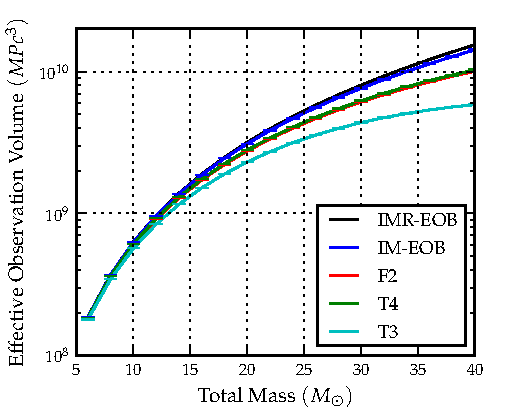
\includegraphics[scale=0.03, clip=false, height=0.28\textheight, width=\columnwidth]{Veffs_logscale_q_1_run03.pdf}}                
  \subfigure[$q=2$]{\label{fig:VeffsLogq2}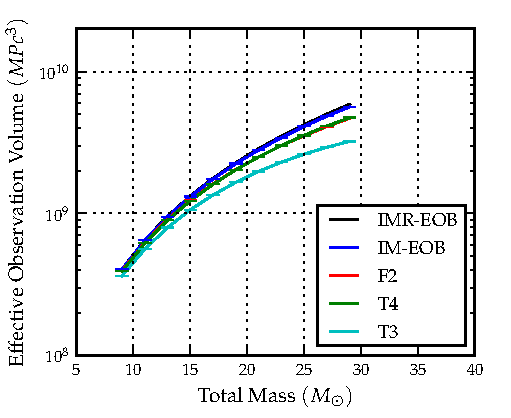
\includegraphics[scale=0.03, clip=false, height=0.28\textheight, width=\columnwidth]{Veffs_logscale_q_2_run03.pdf}}
\\ \subfigure[$q=3$]{\label{fig:VeffsLogq3}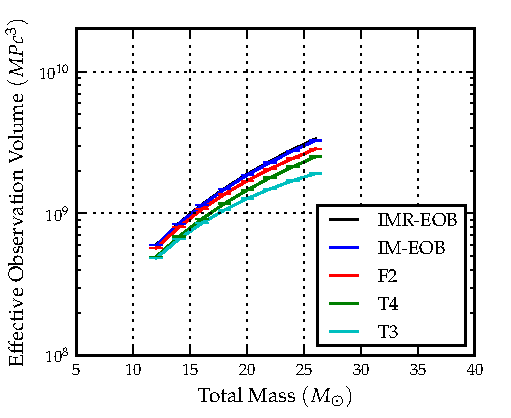
\includegraphics[scale=0.03, clip=false, height=0.28\textheight, width=\columnwidth]{Veffs_logscale_q_3_run03.pdf}}
\subfigure[$q=4$]{\label{fig:VeffsLogq4}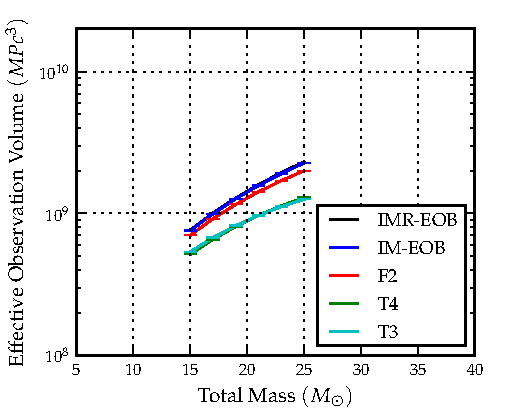
\includegraphics[scale=0.03, clip=false, height=0.28\textheight, width=\columnwidth]{Veffs_logscale_q_4_run03.pdf}}
\\ \subfigure[$q=5$]{\label{fig:VeffsLogq5}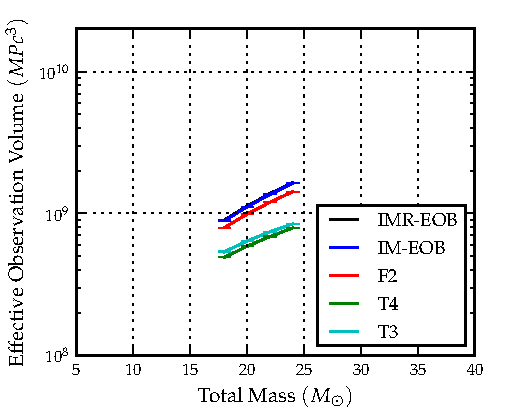
\includegraphics[scale=0.03, clip=false, height=0.28\textheight, width=\columnwidth]{Veffs_logscale_q_5_run03.pdf}}
\subfigure[$q=6$]{\label{fig:VeffsLogq6}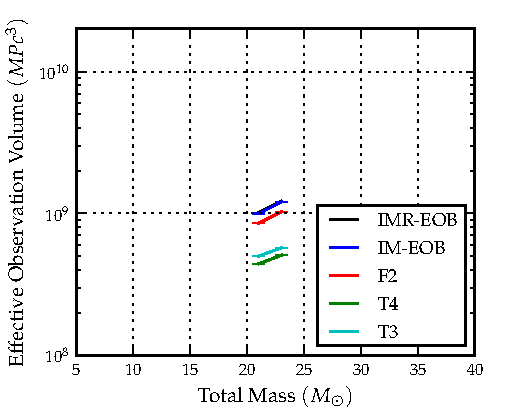
\includegraphics[scale=0.03, clip=false, height=0.28\textheight, width=\columnwidth]{Veffs_logscale_q_6_run03.pdf}}
  \caption{These figures show the variation of the effective observation volume (logarithmic scale) with the total mass of the binary, that would be available to match-filtering searches using different waveform approximants. Each subplot is for a different value of mass ratio $q \l(\equiv m_1/m_2\r)$.}
  \label{fig:VeffsLog}
\end{figure*}
\begin{table}[h]
\caption{\label{tab:maxTotalMassVeff} This table shows the maximum total mass of a system, for each value of the mass-ratio $q$, for which the available effective observation volume using the respective approximant is at least $90\%$ of that accesible with the full IMR EOB waveforms.}
\begin{ruledtabular}
\begin{tabular}{|m{0.18\columnwidth}| m{0.18\columnwidth}| m{0.18\columnwidth}| m{0.18\columnwidth}| m{0.18\columnwidth}|}
mass-ratio & F2 & T4 & T3 & IM EOB\tabularnewline \hline
1 & 16$M_{\odot}$ & 18$M_{\odot}$ & 10$M_{\odot}$ & 40$M_{\odot}$\tabularnewline \hline
2 & 17$M_{\odot}$ & 17$M_{\odot}$ & - & 29$M_{\odot}$\tabularnewline \hline
3 & 18$M_{\odot}$ & - & - & 26$M_{\odot}$\tabularnewline \hline
4 & 19$M_{\odot}$ & - & - & 25$M_{\odot}$\tabularnewline \hline
5 & - & - & - & 24$M_{\odot}$\tabularnewline \hline
6 & - & - & - & 23$M_{\odot}$\tabularnewline \hline
\end{tabular}
\end{ruledtabular}
\end{table}
The furthest that a binary could be located, and be detectable with an SNR of $8$, is called the \textit{horizon distance} $D_{\horizon}$ [citation],
\begin{equation}
D_{\horizon}\equiv D_{\eff}(\rho = 8) = \dfrac{\sigma}{8}.
\end{equation}
The horizon distance defines a two-dimensional spacial surface (horizon) centered at the detector. The effective observation volume is the volume enclosed by this surface (horizon). By definition, all binaries within the effective observation volume, will emit gravitaional radiation that will have an SNR greater than $8$. Following Ref.\citep{FinnChernoffDA} we find the radius of a sphere which has the same volume as the effective volume defined above enclosed within the horizon at SNR $8$. This is ovservation volume that we measure corresponding to the usage of different waveform approximants to model the template waveforms.\newline
Making the assumption that the full IMR EOB model models the nature's waveforms almost perfectly \citep{EOBNRdevel01}, we calculate the horizon distance for a match-filtering search done with IMR EOB template waveforms as
\begin{equation}\label{eq:DhorizonEOB}
D^{\EOB}_{\horizon} = \dfrac{\sigma^{\EOB}}{8} = \dfrac{\sqrt{(g^{\EOB}|g^{\EOB})}}{8},
\end{equation}
where $g^{\EOB}$ has the same meaning as in Eqn.\eqref{eq:handg} if $\tilde{h}(f)$ is the fourier transform of the time domain EOB waveform $h^{\EOB}(t)$. For other approximants, the horizon distance to which a match filtering search can detect using that approximant is the horizon distance the same search could detect to with the exact waveforms (approximated with IMR EOB waveforms), scaled by the fractional loss in signal-to-noise ratio due to the inherent inaccuracy of the approximant. For high SNR, the fractional loss in SNR because of the inherent inaccuracy of the waveform approximant used, is approximated by the mismatch between the waveform generated using the particular approximant and the IMR EOB waveform (for the same binary system). So, the horizon distance to which match-filtering searches can detect gravitational wave signals to using the waveform approximant $\X$ is
\begin{equation}\label{eq:DeffPN}
D^{\X}_{\horizon} = D^{\EOB}_{\horizon}\times\Olap(h^{\X},h^{\EOB}),
\end{equation}
where $\X$ could be the Taylor T3 or the Taylor T4 or the Taylor F2 approximant of just the IM EOB waveforms; and $h^{\X}$ is the waveform generated using approximant $\X$.
%
%Now, to get the effective observation volume for approximant $\X$, we need to find the radius $R_{\eff}$ of the sphere, whose volume equals the volume of space that encapsulates all sources that will be detectable with $\rho\geq 8$. Ref.\citep{FinnChernoffDA} calculates this to be (Eq.(5.1,5.2)):
%\begin{equation}
%\begin{split}
%R_{\eff} = & r_0 \left[3\int_0^{\infty}\D x\,x^2 P(\rho^2(x)\geq\rho_0^2) \right]^{1/3}\\
%\equiv & r_0 \left[3\int_0^{\infty}\D x\,x^2 P(\Gamma\geq x^2) \right]^{1/3}
%\end{split}
%\end{equation}
%where $x$ is the radial parameter of the effective sphere divided by $r_0$, and $r_0$ is a fiducial distance defined in Eq.(5.2a) of Ref.\citep{FinnChernoffDA};
%\begin{subequations}
%\begin{align}\nonumber
%r_0 \equiv & \l(\dfrac{5M^{5/3}\eta f_{7/3}}{96\pi^{4/3}\rho_0^2} \r)^{1/2},\\
%f_{7/3} = &  \int_0^{\infty}\D f \left[f^{7/3} S_n(f) \right]^{-1},\\
%\Gamma = & 16\left[F^2_+\l(1+cos^2\iota\r)/4 + F^2_{\times}cos^2\iota \right],
%\end{align}
%\end{subequations}
%where $f_{7/3} $ is the moment of the power spectral density $S_n(f)$ of the noise in the detector; and $\Gamma$ depends on the antenna patterns of the detector and the inclination angle of the binary, and lies in the range $[0,16]$. Now, if all the sources were optimally oriented, $\Gamma = 16$ always, and $R_{\eff} (\equiv R_{\eff}^{\opt})$ for such a distribution would trivially be equal to $D_{\horizon}$.
%\begin{equation}
%\begin{split}
%R^{\opt}_{\eff} = & r_0 \left[3\int_0^{\infty}\D x x^2 P(\Gamma > x^2) \right]^{1/3},\\
%= & r_0 \left[3\int_0^{4}\D x x^2 \right]^{1/3},\\ 
%= & 4 r_0.
%\end{split}
%\end{equation}
%For a homogenous and isotropic distribution of binary systems in space, however,
%\begin{equation}\label{eq:RisoIntegral}
%\begin{split}
%R^{\iso}_{\eff} = & r_0 \left[3\int_0^{\infty}\D x x^2 P(\Gamma > x^2) \right]^{1/3},\\
%= & (3\times 1.84)^{1/3} r_0.
%\end{split}
%\end{equation}
%The last integral has been numerically evaluated in (see Eq.\eqref{eq:RisoIntegral}) Ref.\citep{FinnChernoffDA}. For the same distribution of sources, the effective observation volume can be written as
%\begin{equation}\label{eq:Veff}
%V_{\eff} = \dfrac{4\pi}{3} R^3_{\eff},
%\end{equation}
%where
%\begin{equation}
%\begin{split}
%R_{\eff} \equiv & R^{\iso}_{\eff},\\ 
%= & \dfrac{(3\times 1.84)^{1/3}}{4} R^{\opt}_{\eff},\\
%\approx & \dfrac{1}{2.26} R^{\opt}_{\eff} = \dfrac{1}{2.26} D_{\horizon}.
%\end{split}
%\end{equation}
The effective observation volume available to a match-filtering search using waveform approximant $\X$,
\begin{equation}
\begin{split}
V^{\X}_{\eff} &= \dfrac{4\pi}{3} \l(\dfrac{D^{\X}_{\horizon}}{2.26}\r)^3,\\
					&= \dfrac{4\pi}{3} \l(\dfrac{D^{\EOB}_{\horizon}}{2.26}\times\Olap(h^{\X},h^{\EOB})\r)^3;
\end{split}
\end{equation}
for a spatially homogenous and isotropic distribution of sources in the universe, where the factor of 2.26 comes from Ref.\citep{FinnChernoffDA}.

Fig.\ref{fig:VeffsLog} shows the variation of the effective observation volume with total mass of the source binary, corresponding to the use of each of the waveform approximants, for certain values of mass-ratio $q(=m_1/m_2)\in\{1,2,3,4,5,6\}$. As we are interested in stellar-mass binary-black-holes, we restrict the individual component masses in the range $(3-20)M_{\odot}$. As a general trend, we observe that the loss in effective observation volume increases with the total mass of the system. For systems more massive than $\sim20M_{\odot}$, all the PN approximants have visibly lower observation volume, as compared to the use of EOB waveforms. 
Table\ref{tab:maxTotalMassVeff} lists the maximum value of the total mass of the system, for each of the PN approximant, for which the loss in the effective observation volume is no more than $10\%$, as compared to EOB waveforms. For example, using Taylor F2 approximant in a match-filtering search for equal-mass systems, leads to a loss in the effective observation volume for those signals of no more than $10\%$ for systems with total mass up to $16M_{\odot}$. For mass-ratio $q\geq 3$, we observe that using both Taylor T4 and Taylor T3 approximants lead to visibly large reduction in the effective observation volume. Also, Taylor F2 approximant can be used to match-filter signals from binary systems with total mass below $\sim 18M_{\odot}$, with less than $10\%$ loss in effective observation volume, and hence the event rate. Taylor T3 approximant has a higher than $10\%$ loss in effective observation volume, across almost the entire designated component-mass range. For systems with total mass above $\sim18M_{\
odot}$, none of the PN approximants can be viably utilized in a match-filtering search.

This indicates that there is a preferential area in the component-mass space, where the computationally inexpensive PN approximants (like Taylor F2) can be used in a match-filtering search. There is also the remaining part of the same space which can only be searched viably using IMR EOB waveforms.
%Similar to Fig.\ref{fig:Olaps}, in the effective observation volume numbers, we observe very small numerical fluctuations. The cause of these is the same as described in Sec.\ref{sec:level2:PNComparison}, and just like in Fig.\ref{fig:Olaps}, the variance of these fluctuations are plotted as errorbars in Fig.\ref{fig:VeffsLog}. Also, the strange behaviour of the T4 waveforms for more asymmetric systems, is also carried over to these figures, and have the same cause as described in Sec.\ref{sec:level2:PNComparison}.


\section{Detection: Bank of PN Waveforms}\label{sec:level1:Effectualness}
\begin{figure}
\centering
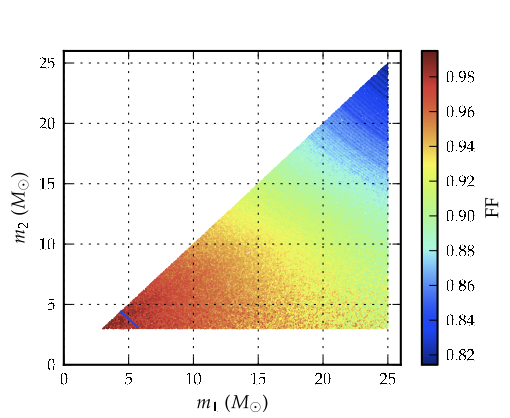
\includegraphics[scale=0.04, clip=false, totalheight=0.3\textheight, width=\columnwidth]{F2EOBeffectualness.pdf}
\caption{\label{fig:match_f2eob_all}This figure shows the effectualness of a bank of Taylor F2 waveforms, with a minimal match of 0.97; at each point in the stellar-mass binary-black-hole region of the component-mass space. The color at each point is the maximum of overlap values between the full IMR EOB waveform for that point and the entire bank of Taylor F2 waveforms.}
\end{figure}
\begin{figure}
\centering
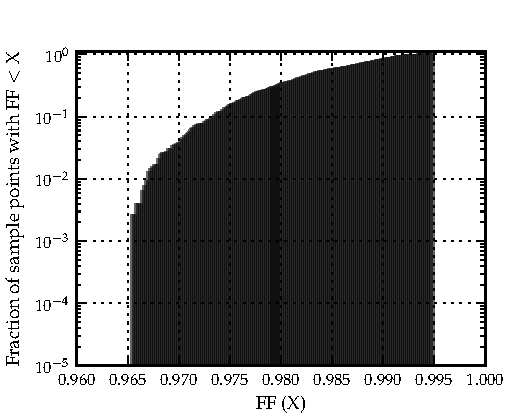
\includegraphics[scale=0.04, clip=false, totalheight=0.3\textheight, width=\columnwidth]{F2EOBhist.pdf}
\caption{\label{fig:cumhist_f2eob_cut14}This figure shows a cumulative histogram of the fraction of the component-mass region, where the bank of Taylor F2 waveforms has an effectualness less than the respective values on the x-axis. For example, over $2\%$ of the component-mass region, the F2 bank has effectualness below $0.97$. The component-mass region shown here has systems with individual component-masses in $(3-20)M_{\odot}$ and total mass below or equal to $14M_{\odot}$.}
\end{figure}
\begin{figure*}[]
\centerline{
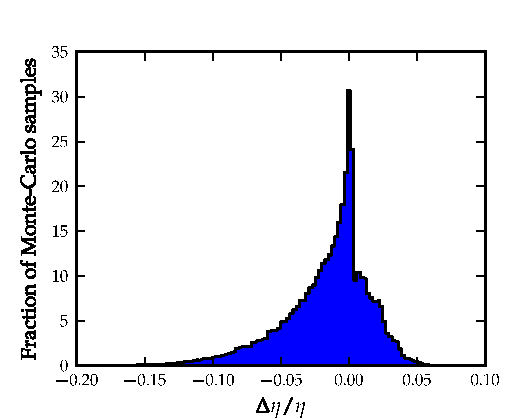
\includegraphics[scale=0.04, clip=false,keepaspectratio=true, width=\columnwidth]{hist_eta_err14paramF2EOB.pdf}\label{fig:errparams_f2eob_eta}              
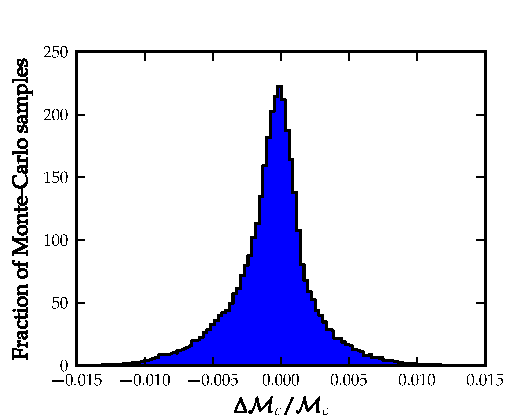
\includegraphics[scale=0.04, clip=false, keepaspectratio=true, width=\columnwidth]{hist_mchirp_err14paramF2EOB.pdf}\label{fig:errparams_f2eob_mchirp}
}
\caption{This figure shows the histogram of fractional difference between the physical parameters recovered by searching for the gravitational-wave signal using Taylor F2 bank of waveforms, and the actual physical parameters of the system used to generate the gravitational-wave signal. The left plot shows the fractional difference in the symmetric mass ratio $\eta$ and the right plot shows the fractional difference in the chirp mass $\mathcal{M}_c$. The designated component-mass-space region is the region with total mass below $14M_{\odot}$ and individual component-masses in $(3-20)M_{\odot}$.}
\end{figure*}

\begin{figure}
\centering
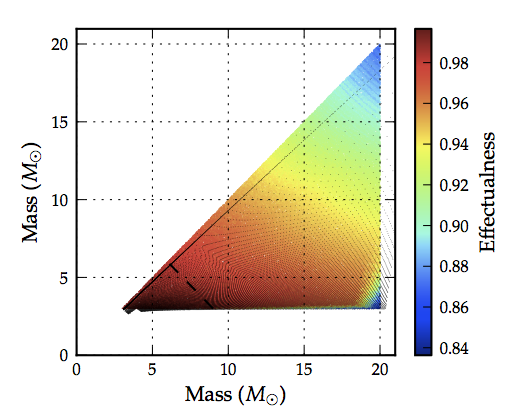
\includegraphics[scale=0.04, clip=false, totalheight=0.3\textheight, width=\columnwidth]{T4EOBeffectualness.pdf}
\caption{\label{fig:match_t4eob_all}This figure shows the effectualness of a bank of Taylor T4 waveforms, with a minimal match of 0.97; at each point in the stellar-mass binary-black-hole region of the component-mass space. The color at each point is the maximum of overlap values between the full IMR EOB waveform for that point and the entire bank of Taylor T4 waveforms.}
\end{figure}
\begin{figure}
\centering
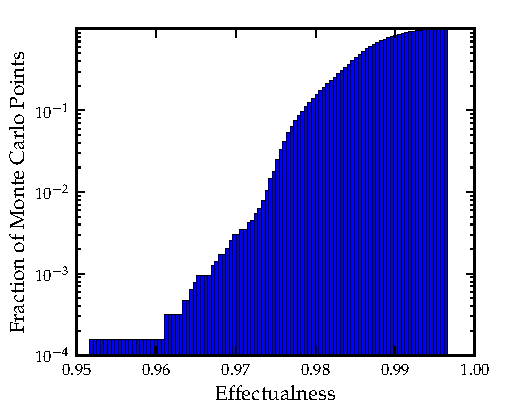
\includegraphics[scale=0.04, clip=false, totalheight=0.3\textheight, width=\columnwidth]{T4EOBhist.pdf}
\caption{\label{fig:cumhist_t4eob_cut10}This figure shows a cumulative histogram of the fraction of the component-mass region, where the bank of Taylor T4 waveforms has an effectualness less than the respective values on the x-axis. For example, over $0.04\%$ of the component-mass region, the T4 bank has effectualness below $0.965$. The component-mass region shown here has systems with individual component-masses in $(3-20)M_{\odot}$ and total mass below or equal to $12M_{\odot}$.}
\end{figure}
\begin{figure*}[]
\centerline{
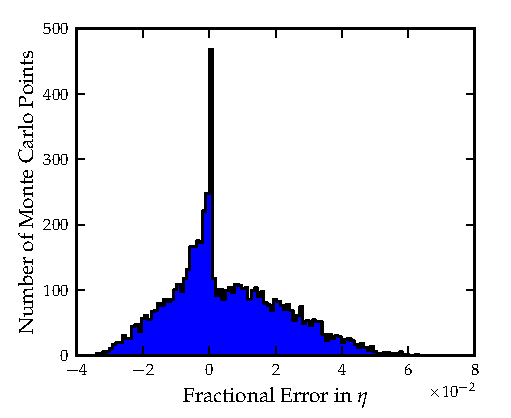
\includegraphics[scale=0.04, clip=false,keepaspectratio=true, width=\columnwidth]{hist_eta_err12paramT4EOB.pdf}\label{fig:errparams_t4eob_eta}              
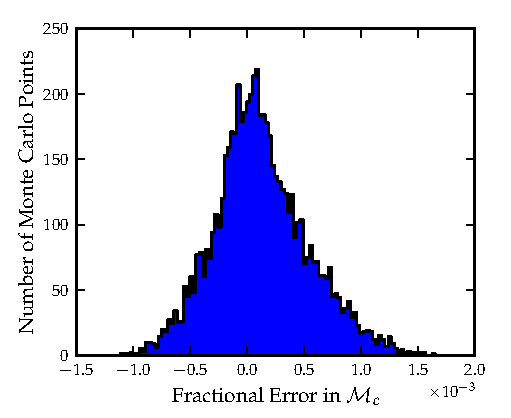
\includegraphics[scale=0.04, clip=false, keepaspectratio=true, width=\columnwidth]{hist_mchirp_err12paramT4EOB.pdf}\label{fig:errparams_t4eob_mchirp}
}
\caption{This figure shows the histogram of fractional difference between the physical parameters recovered by searching for the gravitational-wave signal using Taylor T4 bank of waveforms, and the actual physical parameters of the system used to generate the gravitational-wave signal. The left plot shows the fractional difference in the symmetric mass ratio $\eta$ and the right plot shows the fractional difference in the chirp mass $\mathcal{M}_c$. The designated component-mass-space region is the region with total mass below $12M_{\odot}$ and individual component-masses in $(3-20)M_{\odot}$.}
\label{fig:errparams_t4eob}
\end{figure*}

Following the previous section, in this section we investigate in detail the region in the component-mass space where it suffices to use the PN approximants (Taylor F2 and T4) for match-filtering detection searches, and where using EOB is clearly more viable. In this section, we address this question for searches that use a discrete \textit{bank} \citep{SathyaBankPlacementTauN,SathyaMetric2PN} of waveform templates, as were used in earlier searches done over the intial LIGO data \citep{LSCSearch2004,LSCSearch2005,LSCSearch2008}. As before, the region of the component-mass space that we study is the stellar-mass binary-black-hole region with individual component mass lying in $(3-20)M_{\odot}$.

We do a monte-carlo simulation over the entire stellar-mass binary-black-hole mass region. The simulation was done by generating 100,000 points over the designated region of the component-mass space, uniformly distributed in individual component-mass. We take each of these points, and generate the full IMR EOB waveform for the system with component masses given by the coordinates of the point $a$, starting from the time when the gravitational-wave frequency from the system crosses 15Hz, and ending when the quasi-normal ringing of the final black-hole (formed by the coalescence of the binary) stops. Let $a$ represent a representative point and $h_a^{\EOB}$ be the EOB waveform (shown in superscript) for the point $a$ (shown in the subscript). We also generate a bank of template waveforms of approximant $\X$, using the Owen-Sathya bank placement metric \citep{OwenTemplateSpacing,SathyaBankPlacementTauN,SathyaMetric2PN} to cover the same mass region, with the requirement that the waveform generated for \textit{
any} point $a$ in that mass-region will have a maximized overlap $\geq 0.97$ with \textit{at least} one point in the bank; i.e. $\Olap(h^{\X}_a,h^{\X}_b)\geq 0.97$ for at least one point $h^{\X}_b$ in the aforementioned bank of template waveforms . This is equivalent to saying that the bank has a \textit{minimal match} $\mathrm{MM}$ of $0.97$. Here, $\X$ could be either the Taylor F2 or Taylor T4 waveform approximant.

Given a point $a$ in the component-mass space, and the exact waveform $h^e_a$ generated using the coordinates of the point $a$ as component-masses; the \textit{effectualness} of a bank of template waveforms (of approximant $\X$) is defined as the maximum value of maximized overlap between $h^e_a$ and any member $h^{\X}_b$ of the template waveform bank, i.e.
\begin{equation}
\mathcal{E}(h^e_a|h^{\X}) = \underset{b}{max}\dfrac{(h^e_a|h^{\X}_b)}{\sqrt{(h^e_a|h^e_a)(h^{\X}_b|h^{\X}_b)}}.
\end{equation}
When searching for signals in detector data, the data is match-filtered through the entire bank of waveform templates and the maximum value of the SNR over the entire bank is used in further statistical analysis \citep{LSCSearch2004,LSCSearch2005,LSCSearch2008}. Thus, for a detection search that aims at less than $10\%$ loss in event detection rate, what is required is a bank of template waveforms that has effectualness above $0.965$ over the entire component-mass region that it covers \citep{WaveformAccuracy2008,CompTemplates2009}.

In the monte-carlo simulation over the bank, for every point $a$ we approximate the exact $h^e_a$ with $h^{\EOB}_a$ \citep{EOBNRdevel01}, and calculate the effectualness of the template bank (generated for different waveform approximants) at each of the sample points distributed across the component-mass space.

\subsection{TaylorF2}\label{sec:level2:EffectualnessTaylorF2}
Fig.\ref{fig:match_f2eob_all} shows the effectualness of the Taylor F2 template bank at each point in the component-mass space. We observe a region of the component-mass space where the effectualness of the bank is high enough to not have an event detection rate loss above $10\%$, which corresponds to a minimal effectualness of $0.965$ \citep{WaveformAccuracy2008}. Looking in detail at the region of the space with total-masses below $14M_{\odot}$, we see that in this region of the component-mass space, the bank of Taylor F2 waveform templates has effectualness greater than $0.965$ throughout. This is illustrated by the histogram in Fig.\ref{fig:cumhist_f2eob_cut14}. This cumulative histogram shows the relative fraction of the component-mass-space region (with total mass below $14M_{\odot}$) over which the Taylor F2 waveform template bank has an effectualness below or equal to the value on the x-axis. As can be seen, the Taylor F2 bank has, at all the points sampled in this region, effectualness above $0.965$.
 This corresponds to a maximum loss in event rate of $10\%$ \citep{WaveformAccuracy2008}.

Also, in Fig.\ref{fig:errparams_f2eob}, we can see a histogram of the fractional differences between the true physical mass parameters of a system and the mass parameters of the template waveform in the Taylor F2 bank that has the maximum value of maximized overlap with the IMR EOB waveform for that system. In other words, it shows the fractional error in the mass parameters recovered using a bank of F2 waveform templates. The mass-coordinates we show the errors in are the dimensionless symmetric mass-ratio $\eta$, and the chirp mass $\mathcal{M}_c$,
\begin{equation}
\mathcal{M}_c = M \eta^{3/5}.
\end{equation}
This chirp mass parameter determines the total length in time of the inspiral part of the waveform (to leading order) \citep{SathyaBankPlacementTauN}, and it contains more information than the component-mass parameters. This is also the reason why the chirp mass is recovered with greater precision, as seen in Fig.\ref{fig:errparams_f2eob}. This illustrates that there are no accidental matches of the IMR EOB and Taylor F2 waveforms with very different physical parameters, as the fractional difference between the actual physical parameters of the system and those recovered using the Taylor F2 template bank are $\lesssim 6\%$ for $\eta$ and $\lesssim 0.15\%$ for chirp mass, which are within the expected range [citation].

\subsection{TaylorT4}\label{sec:level2:EffectualnessTaylorT4}
Fig.\ref{fig:match_t4eob_all} shows the effectualness of the Taylor T4 template bank at each point in the component-mass space. As with the Taylor F2 case, we observe a region of the component-mass space where the effectualness of the bank is above the acceptable minimum of $0.965$ \citep{WaveformAccuracy2008}. We found, looking in detail at the region of the space with total-masses below $12M_{\odot}$, that in this region of the component-mass space, the Taylor T4 template bank has effectualness above $0.965$ over more than $99.9\%$ of the region. This is illustrated in Fig.\ref{fig:cumhist_t4eob_cut12}, which shows the fraction of the component-mass region (with total mass below $12M_{\odot}$) where the T4 template bank has an effectualness below the corresponding number on the x-axis. The histogram shows that, over no more than $0.02\%$ of the component-mass area does the effectualness of the T4 template bank drop below $0.965$.

As before, in Fig.\ref{fig:errparams_t4eob}, we show a histogram of the fractional differences between the true physical parameters of a system and the parameters of the template in the Taylor T4 bank that has the maximum value of maximized overlap with the IMR EOB waveform for that system.
This illustrates that there are no accidental matches of the IMR EOB and Taylor T4 waveforms with very different physical parameters, as the fractional difference between the actual physical parameters of the system and those recovered using the Taylor F2 template bank, which are $\lesssim 4\%$ for $\eta$ and $\lesssim 0.1\%$ for chirp mass, are within expected bounds [citation].


\section{Template Placement of EOBNRv2}\label{sec:level1:templateplacement}
\begin{figure}
\centering
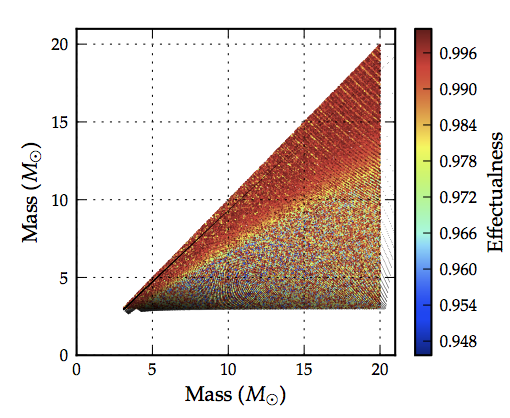
\includegraphics[scale=0.04, clip=false, totalheight=0.3\textheight, width=\columnwidth]{EOBEOBeffectualness.pdf}
\caption{\label{fig:match_eobeob_all}This figure shows the effectualness of a bank of IMR-EOB waveforms, with an intended minimal match of 0.97. The color at each point is the maximum of overlap values between the full IMR EOB waveform for that point and the entire bank of IMR-EOB waveforms.}
\end{figure}
\begin{figure}
\centering
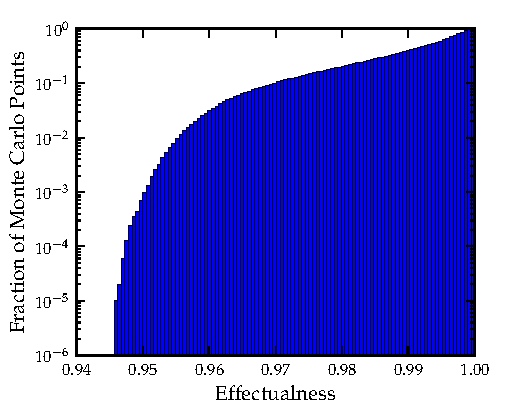
\includegraphics[scale=0.04, clip=false, totalheight=0.3\textheight, width=\columnwidth]{EOBEOBhist.pdf}
\caption{\label{fig:cumhist_eobeob_all}This figure shows a cumulative histogram of the fraction of the component-mass region, where the bank of IMR-EOB waveforms has an effectualness less than the respective values on the x-axis. For example, over $10\%$ of the component-mass region, the IMR-EOB bank has effectualness below the $0.97$. The component-mass region shown here has systems with individual component-masses in $(3-20)M_{\odot}$.}
\end{figure}

In this section we investigate the effectiveness of the Owen-Sathya metric \citep{SathyaMetric2PN}, that was used to generate template banks in data analysis searches in initial LIGO data \citep{LSCSearch2004,LSCSearch2005,LSCSearch2008}, in placing the IMR EOB waveforms. We do a monte-carlo simulation over the entire stellar-mass binary-black-hole region. About 100,000 points were randomly placed throughout the designated region of the component-mass space (uniformly distributed in individual component masses). For each point the effectualness of the IMR EOB template bank was calculated. This is similar to the monte-carlo simulations for Sec.\ref{sec:level1:Effectualness}, only that the approximant used to generate the template bank is also IMR-EOB.

With a bank of template waveforms constructed with an intended minimal match of $0.97$ \citep{BabaketalBankPlacement,SathyaBankPlacementTauN}, we see in Fig.\ref{fig:match_eobeob_all} that the effectualness of the IMR-EOB bank falls quite below the intended value of $0.97$ in a significant portion of the component-mass-space region. This is shown more clearly in the histogram in Fig.\ref{fig:cumhist_eobeob_all}. The cumulative histogram shows the relative fraction of the component-mass-space region over which the IMR-EOB bank has an effectualness below or equal to the value on the x-axis. We observe that over about $10\%$ of the designated region of component-mass space, the IMR-EOB template bank has effectualness below the intended minimum of $0.97$, with the worst values going down to $\sim0.945$. Such low values of effectualness corresponds to a loss in event detection rate of up to $\sim16\%$. Fig.\ref{fig:match_eobeob_all} demonstrates that the template bank generated using the Owen-Sathya bank 
placement metric \citep{OwenTemplateSpacing,SathyaBankPlacementTauN,SathyaMetric2PN,BabaketalBankPlacement} undercovers the component-mass space uniformly across the designated component-mass region. The figure shows narrow regions of low effectualness values, separated by islands of higher effectualness. This pattern is seen to be repeated over most of the component-mass region, and indicates that there is a systematic bias in calculating the \textit{mismatch} between neighbouring templates, while placing the templates.

\section{Conclusion}\label{sec:level1:conclusion}
Studies with effective observation volumes show us that for systems with total mass above $\sim18M_{\odot}$ definitely need to be modelled with the EOB approximant, if one expects to have no more than $10\%$ loss in event detection rate of a match-filtering search. Detailed monte-carlo simulation in the region of the component-mass space with total mass below $18M_{\odot}$ show that discrete banks (constructed using the Owen-Sathya bank-placement metric \citep{SathyaMetric2PN}) of Taylor F2 waveforms can be used to search for gravitational waveforms from binary-black-holes in advanced LIGO, for systems with total mass below $14M_{\odot}$. Also, a template bank of Taylor T4 waveforms can be used, similarly, but only for systems with total mass below $12M_{\odot}$. Above these limits on total mass, the use of EOB waveforms will be much more viable, to have losses in the event-detection-rate less than $10\%$.

The effectiveness of the Owen-Sathya bank-placement metric in placing EOB waveforms, was studied. It was observed that the EOB template bank constructed using this metric with an intended \textit{minimal mismatch} of $0.97$, has effectualness below the intended value for over $10\%$ of the entire binary-black-hole mass-region. The areas where the bank was found to be ineffectual, were observed to be almost uniformly distributed as narrow regions between islands of higher effectualness, suggesting a systematic bias of the metric \citep{SathyaMetric2PN} in estimating the mismatch between neighbouring templates.

% If in two-column mode, this environment will change to single-column
% format so that long equations can be displayed. Use
% sparingly.
%\begin{widetext}
% put long equation here
%\end{widetext}

% figures should be put into the text as floats.
% Use the graphics or graphicx packages (distributed with LaTeX2e)
% and the \includegraphics macro defined in those packages.
% See the LaTeX Graphics Companion by Michel Goosens, Sebastian Rahtz,
% and Frank Mittelbach for instance.
%
% Here is an example of the general form of a figure:
% Fill in the caption in the braces of the \caption{} command. Put the label
% that you will use with \ref{} command in the braces of the \label{} command.
% Use the figure* environment if the figure should span across the
% entire page. There is no need to do explicit centering.

% \begin{figure}
% \includegraphics{}%
% \caption{\label{}}
% \end{figure}

% Surround figure environment with turnpage environment for landscape
% figure
% \begin{turnpage}
% \begin{figure}
% \includegraphics{}%
% \caption{\label{}}
% \end{figure}
% \end{turnpage}

% tables should appear as floats within the text
%
% Here is an example of the general form of a table:
% Fill in the caption in the braces of the \caption{} command. Put the label
% that you will use with \ref{} command in the braces of the \label{} command.
% Insert the column specifiers (l, r, c, d, etc.) in the empty braces of the
% \begin{tabular}{} command.
% The ruledtabular enviroment adds doubled rules to table and sets a
% reasonable default table settings.
% Use the table* environment to get a full-width table in two-column
% Add \usepackage{longtable} and the longtable (or longtable*}
% environment for nicely formatted long tables. Or use the the [H]
% placement option to break a long table (with less control than 
% in longtable).
% \begin{table}%[H] add [H] placement to break table across pages
% \caption{\label{}}
% \begin{ruledtabular}
% \begin{tabular}{}
% Lines of table here ending with \\
% \end{tabular}
% \end{ruledtabular}
% \end{table}

% Surround table environment with turnpage environment for landscape
% table
% \begin{turnpage}
% \begin{table}
% \caption{\label{}}
% \begin{ruledtabular}
% \begin{tabular}{}
% \end{tabular}
% \end{ruledtabular}
% \end{table}
% \end{turnpage}

% Specify following sections are appendices. Use \appendix* if there
% only one appendix.
%\appendix
%\section{}
%\FloatBarrier
% If you have acknowledgments, this puts in the proper section head.
\begin{acknowledgments}
We thank NSF grants PHY-1040231 and PHY-0600953, for support with the computational resources needed for this work.
\end{acknowledgments}

% Create the reference section using BibTeX:
\bibliography{bank_effectualness_study}

\end{document}
%
% ****** End of file apstemplate.tex ******

